%------------------------------------------------------------------------
%Editar Diplomado
\hypertarget{cv:eliminarPantalla}{\section{Eliminar Pantalla(PENDIENTE DE PANTALLAS)}} \label{sec:eliminarPantalla}

	Esta funcionalidad le permitirá eliminar una pantalla innecesaria o incorrecta. Para eliminar una pantalla es necesario que no se encuentre asociado a casos de uso, al igual que sus acciones.

		\subsection{Procedimiento}

			%Pasos de procedimiento
			\begin{enumerate}
	
			\item Oprima el botón \IUBotonEliminar{} de un registro existente de la pantalla \ref{fig:GestionarPantallas} ''Gestionar Pantallas''.
	
			\item Se mostrará el mensaje \ref{fig:confirmaEliminaPantalla} sobre la pantalla \ref{fig:GestionarPantallas} ''Gestionar Pantallas''.
			
			%Pantalla
			\begin{figure}[htbp!]
				\begin{center}
					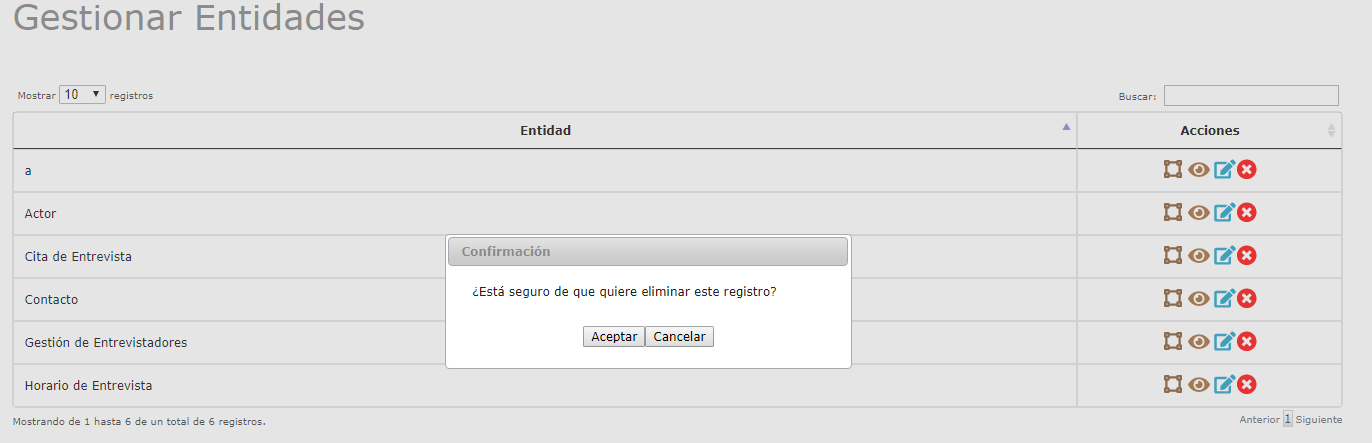
\includegraphics[scale=0.5]{roles/lider/entidades/pantallas/IU12-3MSG10}
					\caption{MSG de Confirmación}
					\label{fig:confirmaEliminaPantalla}
				\end{center}
			\end{figure}
						
			\item Oprima el botón \IUAceptar.
			
			\item Se mostrará el mensaje \ref{fig:pantallaEliminada} en la pantalla \ref{fig:GestionarPantallas} ''Gestionar Pantallas''.
			
			\begin{figure}[htbp!]
				\begin{center}
					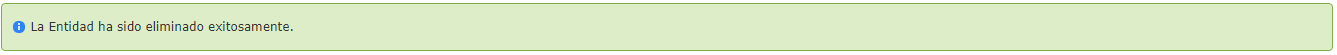
\includegraphics[scale=0.5]{roles/lider/entidades/pantallas/IU12-3MSG1}
					\caption{MSG: Pantalla Eliminada}
					\label{fig:pantallaEliminada}
				\end{center}
			\end{figure}
			\end{enumerate}